%%
%% This is file `sample-sigconf.tex',
%% generated with the docstrip utility.
%%
%% The original source files were:
%%
%% samples.dtx  (with options: `sigconf')
%% 
%% IMPORTANT NOTICE:
%% 
%% For the copyright see the source file.
%% 
%% Any modified versions of this file must be renamed
%% with new filenames distinct from sample-sigconf.tex.
%% 
%% For distribution of the original source see the terms
%% for copying and modification in the file samples.dtx.
%% 
%% This generated file may be distributed as long as the
%% original source files, as listed above, are part of the
%% same distribution. (The sources need not necessarily be
%% in the same archive or directory.)
%%
%% Commands for TeXCount
%TC:macro \cite [option:text,text]
%TC:macro \citep [option:text,text]
%TC:macro \citet [option:text,text]
%TC:envir table 0 1
%TC:envir table* 0 1
%TC:envir tabular [ignore] word
%TC:envir displaymath 0 word
%TC:envir math 0 word
%TC:envir comment 0 0
%%
%%
%% The first command in your LaTeX source must be the \documentclass command.
\documentclass[sigconf]{acmart}
%% NOTE that a single column version is required for 
%% submission and peer review. This can be done by changing
%% the \doucmentclass[...]{acmart} in this template to 
%% \documentclass[manuscript,screen]{acmart}
%% 
%% To ensure 100% compatibility, please check the white list of
%% approved LaTeX packages to be used with the Master Article Template at
%% https://www.acm.org/publications/taps/whitelist-of-latex-packages 
%% before creating your document. The white list page provides 
%% information on how to submit additional LaTeX packages for 
%% review and adoption.
%% Fonts used in the template cannot be substituted; margin 
%% adjustments are not allowed.

%%
%% \BibTeX command to typeset BibTeX logo in the docs
\AtBeginDocument{%
  \providecommand\BibTeX{{%
    \normalfont B\kern-0.5em{\scshape i\kern-0.25em b}\kern-0.8em\TeX}}}

%% Rights management information.  This information is sent to you
%% when you complete the rights form.  These commands have SAMPLE
%% values in them; it is your responsibility as an author to replace
%% the commands and values with those provided to you when you
%% complete the rights form.
\setcopyright{acmlicensed}
\copyrightyear{2018}
\acmYear{2018}
\acmDOI{XXXXXXX.XXXXXXX}

\usepackage{todonotes}

%% These commands are for a PROCEEDINGS abstract or paper.
\acmConference[EEC289Q]{Make sure to enter the correct
  conference title from your rights confirmation emai}{March 20, 2024}{Davis, CA}
%
%  Uncomment \acmBooktitle if th title of the proceedings is different
%  from ``Proceedings of ...''!
%
%\acmBooktitle{Woodstock '18: ACM Symposium on Neural Gaze Detection,
%  June 03--05, 2018, Woodstock, NY} 
\acmISBN{978-1-4503-XXXX-X/18/06}


%%
%% Submission ID.
%% Use this when submitting an article to a sponsored event. You'll
%% receive a unique submission ID from the organizers
%% of the event, and this ID should be used as the parameter to this command.
%%\acmSubmissionID{123-A56-BU3}

%%
%% For managing citations, it is recommended to use bibliography
%% files in BibTeX format.
%%
%% You can then either use BibTeX with the ACM-Reference-Format style,
%% or BibLaTeX with the acmnumeric or acmauthoryear sytles, that include
%% support for advanced citation of software artefact from the
%% biblatex-software package, also separately available on CTAN.
%%
%% Look at the sample-*-biblatex.tex files for templates showcasing
%% the biblatex styles.
%%

%%
%% The majority of ACM publications use numbered citations and
%% references.  The command \citestyle{authoryear} switches to the
%% "author year" style.
%%
%% If you are preparing content for an event
%% sponsored by ACM SIGGRAPH, you must use the "author year" style of
%% citations and references.
%% Uncommenting
%% the next command will enable that style.
%%\citestyle{acmauthoryear}

%%
%% end of the preamble, start of the body of the document source.
\begin{document}

%%
%% The "title" command has an optional parameter,
%% allowing the author to define a "short title" to be used in page headers.
\title{EEC289Q - Optimal uop Scheduling}

%%
%% The "author" command and its associated commands are used to define
%% the authors and their affiliations.
%% Of note is the shared affiliation of the first two authors, and the
%% "authornote" and "authornotemark" commands
%% used to denote shared contribution to the research.

\author{Aiden Grossman}
\affiliation{%
  \institution{UC Davis}}
\email{amgrossman@ucdavis.edu}

%%
%% By default, the full list of authors will be used in the page
%% headers. Often, this list is too long, and will overlap
%% other information printed in the page headers. This command allows
%% the author to define a more concise list
%% of authors' names for this purpose.

%%
%% The abstract is a short summary of the work to be presented in the
%% article.
\begin{abstract}
While executing instructions, modern superscalar processors decode instructions into one or more
micro-operations (uops) that are then executed on an individual execution unit. CPUs typically have
several execution units, with each one being specialized to only execute certain types of uops. However,
this decomposition into uops creates a scheduling problem: namely how the uops should get scheduled onto
the execution ports to minimize the number of cycles needed to execute a block of instructions. Due to the
many constraints necessitated by being in silicon, CPUs often use heuristic based algorithms to assign uops
to slots and ports. The use of these heuristics ultimately raises the following question: how much headroom
is being given away by these suboptimal heuristics? By using ILP to optimally schedule uops, we find that
optimal uop schedules decrease the number of cycles needed for uop execution for a basic block by approximately
20\%. These results demonstrate that there is potentially significant headroom gained by global context and
better scheduling that could potentially be exploited by better heuristics. We anticipate this study to be
useful on a general information level to those designing CPUs, guiding them on where potential performance
improvements are, and to be a starting point for more sophisticated models of the uop-scheduling problem
specifically and to other portions of the full CPU pipeline.
\end{abstract}

%%
%% Keywords. The author(s) should pick words that accurately describe
%% the work being presented. Separate the keywords with commas.
\keywords{CPU, Optimal, ILP, Scheduling, Cost-modeling}

\received{20 February 2007}
\received[revised]{12 March 2009}
\received[accepted]{5 June 2009}

%%
%% This command processes the author and affiliation and title
%% information and builds the first part of the formatted document.
\maketitle

\section{Introduction}

\begin{table*}[t]
\begin{tabular}{|c|c|c|c|}
\hline
Tool & Target & MAPE & Tau \\
\hline
\hline
uiCA \cite{abel2022uica} & Inverse throughput & 1.91\% & 0.9612 \\
\hline
OSACA \cite{laukemann2018osaca} & Inverse throughput (roofline) & 36.85\% & 0.5311 \\
\hline
llvm-mca \cite{dibiagio2018mca} & Inverse throughput & 22.67\% & 0.8069 \\
\hline
GRANITE \cite{sykora2022granite} & Inverse throughput & 6.67\% & Not Available \\
\hline
Ithemal \cite{mendis2019ithemal} & Inverse throughput & 8.34\% & Not Available \\
\hline
\end{tabular}
\caption{A comparison of the various cost modeling tools based on the BHive data set. In this case, MAPE refers to mean
average percent error between the predicted value and the ground truth value. Tau refers to Kendall's tau, which describes
how well the tool ordered all entries relative to each other, with 1.0 being a perfect ordering. These results are
specifically on the sandy bridge microarchitecture.}
\end{table*}

While GPUs been been a recent focus due to the recent AI/ML rush, CPUs are still the backbone of most
modern computing. Understanding how modern workloads are impacted by the microarchitectural details of
modern CPUs is becoming increasinbly important to improve performance \cite{moseley2015warehouseprofiling}.
This is especially true as we are beginning to get to the end of Moore's law, and need to resort to other
techniques, like better compiler optimizations, to continue to improve performance \cite{lattner2020mlir}.
Instead of being able to rely on physical improvements like Dennard Scaling to enable more transistors with lower
power to run at higher clock frequencies without too many adjustments to the microacrchitecture, we need to begin
thinking about how to use the resources that we have, both from the software side utilizing the hardware, and the
hardware itself making efficient usage of the underlying standard cells and other building blocks if we want
to continue to improve performance.
While techniques to make software run more efficiently on current microarchitectures have shown a lot of
promise recently, there is also potential headroom within the CPU design
itself. This headroom can come in a variety of areas, such as cache replacement heuristics \cite{moseley2023emissary},
and from other areas, including uop scheduling.

Performing a headroom analysis (the aim of this study) on a specific aspect of a system, like a full CPU, allows
for the analysis of bottlenecks by assuming a specific task is performed optimally. This has been done before in
several contexts, especially compilers \cite{doerfert2023oraql} \cite{lozano2019combinatorialregalloc}. While these
headroom analyses can not immediately be deployed due to either correctness constraints or runtime constraints,
but they can be incredibly useful in showing how good the heuristics in a production system are compared to the
optimal solution, which can help guide efforts and what should be improved by showing what areas could potentially
benefit from better heuristics, and also quantify on an absolute scale how good a system is.

\begin{figure*}[t]
  \centering
  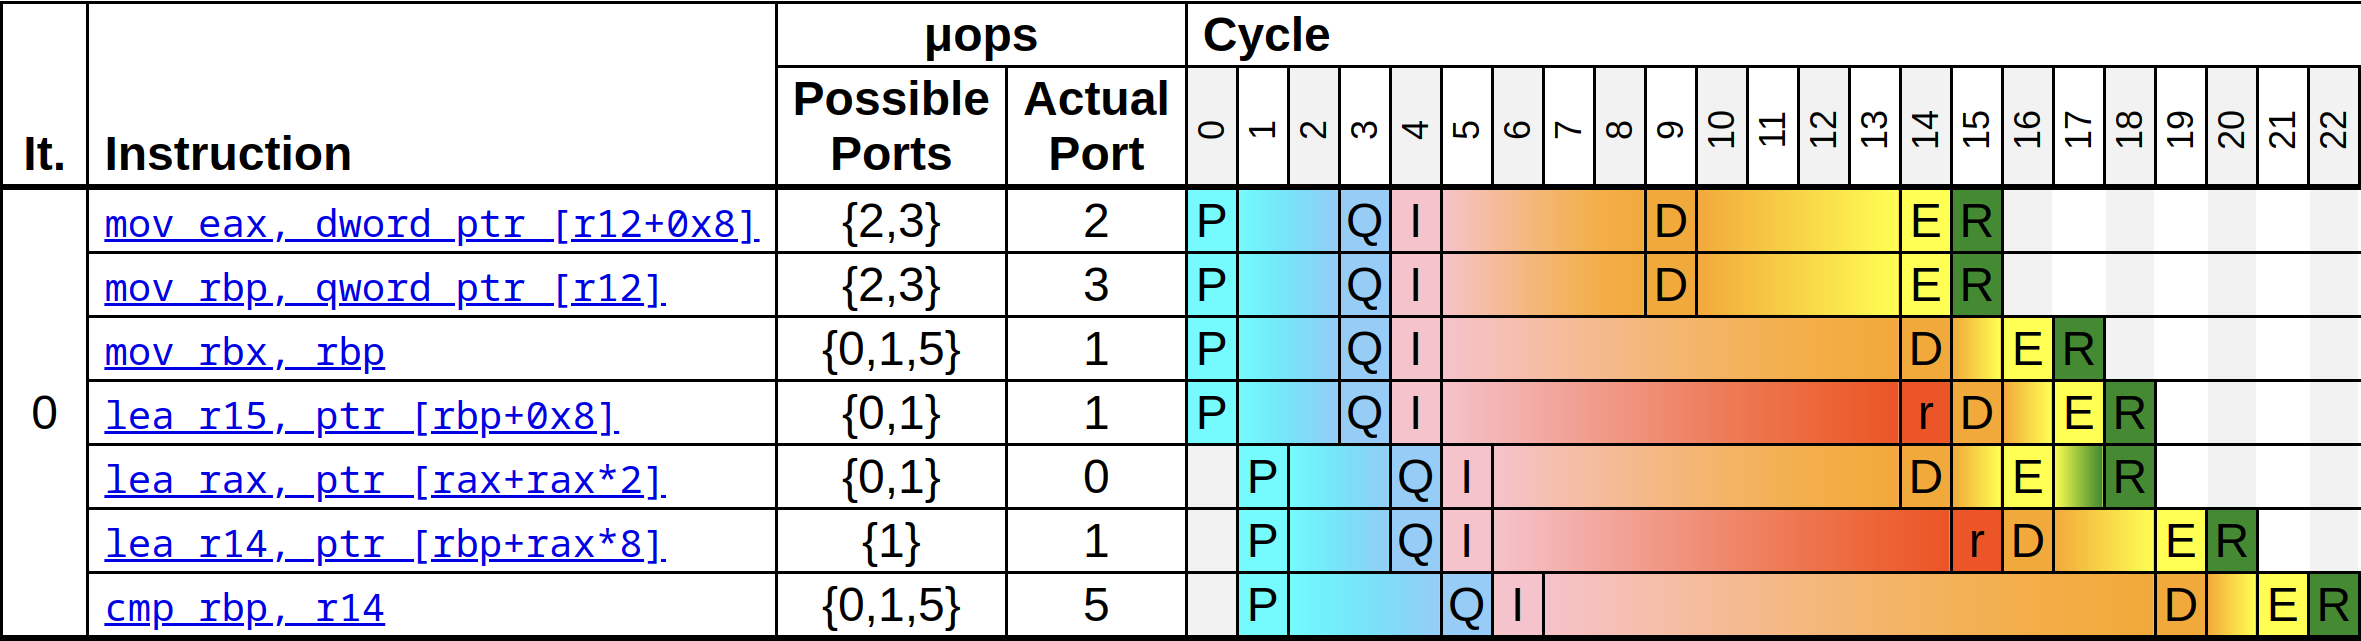
\includegraphics[width=\linewidth]{uica_trace.png}
  \caption{The schedule for this basic block as reported by uiCA, with the total time taking for uop execution (from the first
  dispatch to the last execution) being 12 cycles. The orange D blocks indicate the cycle a uop is dispatched to an execution
  port and the yellow E blocks represent the cycle a uop finishes executing.}
  \label{figure:uica-trace}
\end{figure*}

\section{Background}

Modern superscalar CPUs decode instructions into one or more micro-operations (uops) that can be executed
independently, assuming that their dependencies are available. The uop scheduling is handled by the renamer,
so-called because it "renames" registers while mapping architectural registers to physical registers on the CPU
\cite{abel2022uica} \cite{fog2023architecture}. The renamer will allocate instructions to ports using a pressure-based
algorithm. After the renamer assigns a uop to a port, it goes to that execution port's scheduler, which will then
dispatch it into the port once all of its dependencies have been satisfied \cite{abel2022uica}. Each uop will have a set
of execution ports that it can be assigned to. For example, on Intel's Sandy Bridge microarchitecture, most general
integer operations can be issued to ports 0, 1, or 5, as they contain ALUs. Other more specialized operations, like
integer multiplies, can only be assigned to specific ports, port 1 in the case of integer multiplication, due to
latency constraints (integer multipliation needs three cycles compared to the one cycle needed for most instructions)
and the additional circuitry needed for those special operations \cite{fog2023architecture}. In addition to assigning
micro-operations to specific ports given availability and port-constraints and mapping architectural registers to
physical registers, the renamer also executes certain uops itself. For example, register zeroing idioms like
\texttt{xor \%rax, \%rax} will be recognized by the renamer and executed within the renamer rather than being
dispatched to an execution port. This also allows the renamer to break dependencies between uops with zeroing
idioms between them as even though they might be using the same architectural register, they are not dependent
and can be mapped to different physical registers.

Due to the inherent complexity of modern CPUs, the need to extract as much performance as possible, and the lack
of quality documentation available from CPU vendors, a variety of projects have attempted to model modern CPUs,
Intel X86 CPUs in particular, to a cycle-accurate level for these reasons. There have been several analytical
simulators with various target metrics and various levels of performance including OSACA \cite{laukemann2018osaca},
llvm-mca \cite{dibiagio2018mca}, uiCA \cite{abel2022uica}, and Facile \cite{abel2023facile}. These tools have varying
models of the underlying pipeline that attempt to model the CPU and have various degrees of accuracy as showcased in
REFERENCE TO TABLE 1 HERE. These tools also need a substantial amount of data to model a modern X86 pipeline correctly,
particularly which instructions decompose into what uops, the throughput and latencies of each instruction, and other
information, such as what instructions can be macro or micro fused with each other. This information can be obtained
from the architectural manuals provided by Intel and AMD, or through benchmarking \cite{abel2019uopsinfo}
\cite{courbet2018exegesis}. llvm-mca get its information from the LLVM \cite{lattner2004llvm} scheduling models,
which are updated manually using information from the CPU vendors (either contributed by employees with access to
internal information, or using external information from the architectural manuals), or from benchmarking tools
like uops.info \cite{abel2019uopsinfo}, or the purpose-built llvm-exegesis \cite{courbet2018exegesis}. While the model
of the CPU pipeline matters a lot, having accurate data is also a significant contributor to accuracy, so much so
that custom benchmarking tools using specialized techniques like kernel-mode benchmarking have been purpose-built to
solve this problem \cite{abel2020nanobench}.

\begin{figure*}[t]
  \centering
  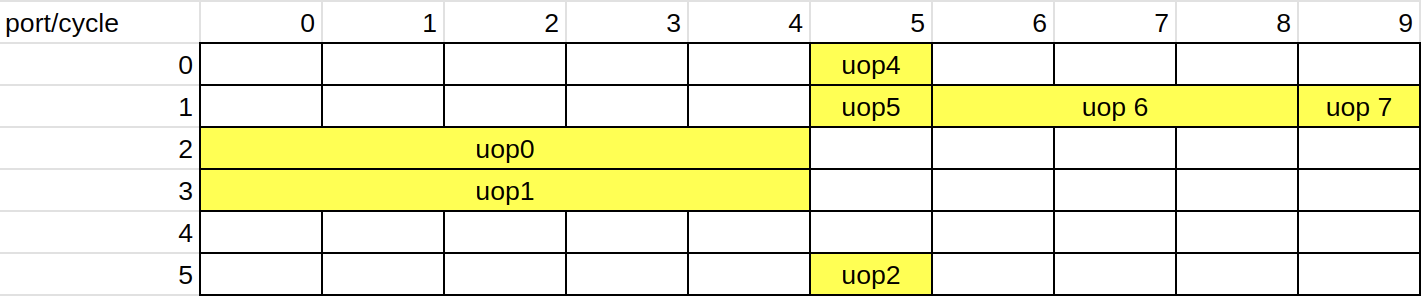
\includegraphics[width=\linewidth]{optimal_schedule.png}
  \caption{The optimal schedule for the block shown in the uiCA trace in figure \ref{figure:uica-trace}. In this case,
  the ILP solver found an optimal solution for the scheduling problem with a total time of ten cycles, two less than
  the actual schedule.}
  \label{figure:optimal-schedule}
\end{figure*}

These projects most often attempt to the model the throughput of an individual \textit{basic block}, or a
control-flow free sequence of instructions. This means that more complex conditions like branches don't need
to be modeled, while still allowing beyond-basic block information to be obtained by aggregating information
from multiple basic blocks.

It is important to note that these simulators also make quite a number of assumptions about the execution context
when providing results. They assume that every single memory access will result in a L1 cache hit. In addition,
they assume that the CPU frontend (mainly instruction decode) is working optimally and doesn't starve the backend,
within some limits. In addition, it is assumed there are no exceptions/interrupts thrown during execution (e.g.,
TLB lookups), that there are no branch mispredictions when executing a loop, and that certain floating point
conditions that can lead to increased latency for certain instructions never occur \cite{abel2022uica}. These
assumptions often do not hold in the real world, but for the analysis of compute-bound basic blocks, these
assumptions are reasonable.

While these simulators are not aimed at being used for exploring CPU hardware level headroom questions, they can
be modified to do so and provide a strong base to do so. Many of the issues that need to be solved are common,
such as obtaining the uop decomposition of instructons, and modeling dependencies between uops.

\section{Methods}

\subsection{Obtaining Baseline Performance Results}

In order to obtain baseline performance results, we used uiCA \cite{abel2022uica}. We chose not to use the
underlying performance information from a dataset like BHive as we are only modeling the uop execution
phase rather the exeuction of the complete instruction. It is extremely difficult to obtain the number of cycles
solely used for port execution in modern CPUs as it necessitates the use of a tool like Brandon Falk's SushiRoll
\cite{falk2019sushiroll}, a custom research kernel aimed at deterministic low-level execution. These techniques are
difficult to use, only support specific hardware, and produce results for which there is no automated tooling
to extract the required information needed for this project.

uiCA is aimed at finding the throughput of an individual basic block executed in steady state. However,
specific details about conditions within the CPU microarchitecture during the execution of each iteration are
available in a JSON format. To get only the time used for uop execution (within a single iteration), we
take the cycle of when the last uop in the iteration finishes executing, and the cycle when the first uop in
the iteration is dispatched, and then find the difference to get the time of uop execution. An execution trace
from uiCA exemplifying this is shown in figure \ref{figure:uica-trace}. This is not a perfect
strategy as it doesn't take into account other conditions like instruction decode, but works reasonably enough.

uiCA, being a static cost model, also is not a perfect representation of the CPU pipeline. However, from testing,
uiCA is quite accurate, on average obtaining results within 1-2\% of ground truth values, meaning it is reasonably
accurate in practice at scale. It was also extensively validated during development against ground truth data
obtained using highly accurate kernel-mode microbenchmarks to reverse engineer the underlying microarchitecture, so
while it is not a perfect model, it is accurate enough for the purposes of this study.

\subsection{Obtaining Optimal Performance Results}

To obtain optimal performance results, we again used uiCA, but this time a modified version aimed at also
exposing the uop decomposition of each instruction and the dependencies between each instruction. To do this,
we modified uiCA to emit a JSON file containing all of the uops for a specific basic block and all the register
dependencies between them. This ignores flag dependencies, but this does not impact many basic blocks. After
running uiCA on an individual basic block with our modifications, we are able to use the JSON output in another
tool that sets up and solves an ILP instance as described in section \ref{sec:ilp-formulation}. Once the ILP instance
is solved, we are able to report the objective, which is the cycle the last uop finishes executing. The optimal solution
for the uiCA trace shown in figure \ref{figure:uica-trace} is shown in figure \ref{figure:optimal-schedule}.

\subsection{Data Collection}

\begin{figure*}[t]
  \centering
  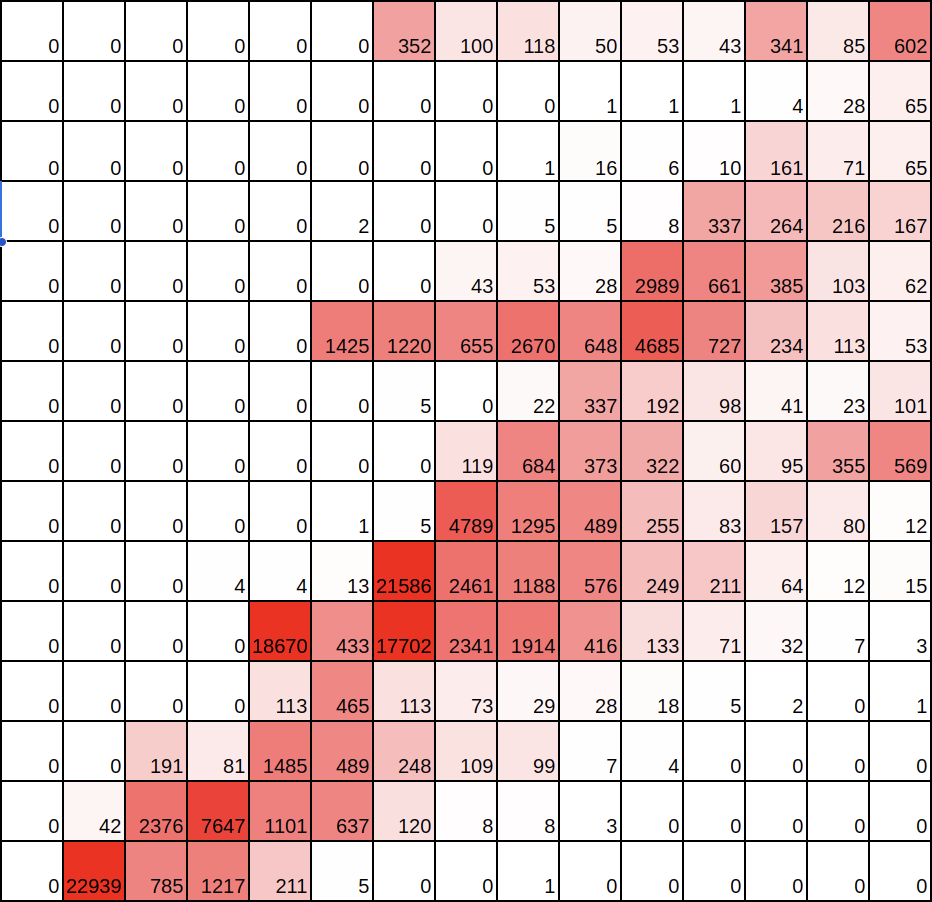
\includegraphics[width=0.6\linewidth]{confusion_matrix.png}
  \caption{A confusion matrix comparing the results obtained from uiCA with the results obtained from the ILP
  instances. The x-axis is the number of cycles that uiCA used while the y-axis is the number of cycles that
  our ILP formulation found. The number in each block is colored according to a gradient scale, with each
  number begin the number of times that cycle pair was recoreded.}
  \label{figure:confusion-matrix}
\end{figure*}

For obtaining data, we use a subset of the BHive \cite{chen2019bhive} dataset of basic blocks that was modified as
a part of analysis on uiCA \cite{abel2022uica} to improve its accuracey and to remove blocks that didn't match
the modeling assumptions listed in part 1. The BHive dataset is composed of basic blocks extracted using runtime
instrumentation from a variety of sources such as Clang/LLVM and OpenBLAS. These basic blocks were further filtered
as part of the uiCA evaluation to remove blocks that could potentially run into memory aliasing, which requires
more complex modeling of memory constraints as a memory store needs to propagate before that address can be
loaded again, requiring complex value-specific modeling of aliasing information that is not covered by tools at this
level. In addition, some results were removed due to being impossible in reality, implying a false measurement. This
is useful for other tools, but does not concern us as we are not using the benchmark results from BHive. Finally,
other blocks were removed for reasons like unbalanced X87 stack operations, which cause a number of modeling issues.

To obtain the comparison data, we wrote a script that iterated over the entire dataset in parallel, finding the baseline
performance results using uiCA and a custom script to find the number of cycles between the execution of the last uop
and the dispatch of the first uop, and solving the ILP instance given the uop decomposition and dependency information
emitted from our modified version of uiCA for each basic block within the dataset. If a basic block did not conform to
our modeling expectations (certain optimizations were performed, creating zero latency uops, or a single uop had multiple
different latencies for each of its output operands), uiCA threw an error and our dataset iterator script simply
discarded it. There were also several instances of the ILP instance for a specific basic block timing out. When this
occurred, we simply took the incumbent solution after the timeout was reached.

We only obtained results for one specific microachitecture, Sandy Bridge, mostly due to familiarity with the
microarchitectural details and hardware access in case some edge case came up where benchmarking would have been
useful.

\section{ILP Formulation}
\label{sec:ilp-formulation}

There are several constraints that need to be met in order for a uop schedule to be valid. Uops that have dependencies
must start after their dependencies have finished executing, uops cannot execute on the same port at the same time,
and a uop can only be scheduled to an execution port that is able to execute it. We setup the ILP instance by modeling
dependency constraints and taking inspiration from a ILP setup for multicore scheduling to model port-execution
constrants \cite{ying2009multicoreilp}. To this end, we define the following variables:

\begin{enumerate}
    \item $x_i$ - The start cycle of uop $i$. This is restricted to being an integer within the ILP model.
    \item $\ell(i)$ - The latency of uop $i$. This will always be an integer as it is an input to the model.
    \item $d_{ii'j}$ - If tasks $i$ and $i'$ are assigned to the same execution port $j$ and $i$ starts execution before $i'$, this binary variable is one, and it is zero otherwise (or not created in the model at all).
    \item $p_{ij}$ - This binary variable is set to one if uop $i$ is executing on port $j$, and it is zero otherwise.
    \item $m$ - An unconstrainted variable.
    \item $P$ - The set of ports that the microarchitecture has.
    \item $U$ - The set of uops in the basic block.
    \item $M$ - An arbitarily large value used for implementing M constraints.
\end{enumerate}

Using these variables, we define the following constraints:

\begin{enumerate}
    \item For every dependency edge where uop $i$ depends on uop $i'$: $x_i>x_{i'}+\ell(i')$.
    \item $$\forall i \in U : x_i + \ell(i) < m$$
    \item $$\forall i \in U : \sum^{j \in P} p_{ij}=1$$
    \item For every port $j$ that uop $i$ cannot execute on: $p_{ij}=0$
    \item For every pair of uops ($i$ and $i'$) that are both assigned to the same port $j$ (i.e., $p_{ij}=p{i'j}=1$,
    $$x_i+\ell(i)\leq x_{i'}+(1-d_{ii'j})M$$
    $$x_{i'}+\ell(i')\leq x_{i}+d_{ii'j}M$$
\end{enumerate}

For the optimization objective, we do the following:

$$\min{m}$$

The first three constraints are able to be expressed as classical ILP constraints. The last constraint is expressed
as an indicator constraint as it only needs to apply when both uops are assigned to the same port. This is easily done
within Gurobi, which is then able to use branch and bound techniques to solve the now non-convex ILP instance. This constraint
uses a so-called Big M constraint and an additional variable ($d_{ii'j}$) to express the idea that only one of the constraints
has to hold. In this case, it means that the uops can be scheduled on either side of each other, but still can't conflict.
The $m$ variable is essentially the maximum variable. We optimize over this variable so that we can minimize the last cycle
of the last uop, which would not be possible without an additional variable.

For several of these constraints, we also only enumerate a small number of them to try and reduce the complexity of the ILP
instance. For example for the second constraint, for every uop $i$, we only need to create a binary port assignment variable,
$p_{ij}$ for every uop that the port can run on rather than every uop that exists within the microarchitecture. Similarly for
four, we only need to create a variable $d_{ii'j}$ for every possible intersection of ports. If we naively iterated over every
possible uop with every single other uop, we would potentially end up with $n^2p$ variables where $n$ is the number of uops
and $p$ is the number of architectural ports. By only iterating over the actual conflicts, we reduce the number of variables
significantly as within a basic block there are usually only tens of instructions at most that all can only execute on
specific ports, making the instance size tractable with this optimization.

\section{Results}

Using the methodology described above, we were able to obtain data on 142642 basic blocks out of 192430 basic blocks.
49788 basic blocks did not meet our modeling constraints (had uops with latencies that were variable between output
operands or went through register renmaing and had uops with zero latencies). Out of the 142642 basic blocks, the ILP solver
timed out on 24 instances, thus making the successful number of solves at 99.98\%. The 24 instances where it failed, we were
still able to obtain a valid solution, it was just not provably optimal. Within the set of blocks that matched out
modeling criteria, we saw an average improvement over the baseline with the optimal solution of 23.09\%. In some cases,
the optimal solution performed worse than the baseline solution due to a lack of modeling certain optimizations that
uiCA does model.

The results are easily summarized in the confusion matrix shown in figure \ref{figure:confusion-matrix}. We can see that
there are some common instances where the ILP solver does end up getting a value worse than the baseline due to the
previously mentioned issues. However, we see the solver most of the time either matching the baseline number of finding
values that are somewhat less than the baseline values. This is consistent with the rest of the results, and the idea
that there is a some headroom attainable from this optimization.

\section{Limitations}

There are several limitations to this work. First off, we are not implementing several optimizations that the CPU
performs that could potentially decrease latency. Second, the definition of uop execution time is slightly crued,
and there is no good way to measure it. To be able to better say that optimal uop scheduling is a bottleneck, a model
would need to take into account much more of the CPU pipeline, such as instruction decode as uops cannot be dispatched
before they have been decoded, and some longer basic blocks, or blocks with complex instructions, will end up being decoded
over several cycles, and the first instructions to be decoded will be able to execute their uops before other instructions
have even finished decoding.

To simplify the creation of uop latency and dependency information for individual basic blocks, we are also not currently
modeling dependencies between flag registers. While many basic blocks do not have instructions that depend on the values
of flag registers (e.e.g, those with just integer arithmetic and/or register move operations), but many will, like those
containing the \texttt{cmov} instruction, which needs the flag values from a previous instruction to decide whether
or not to move a value.

In addition, there are other edge cases that we are not currently considering, like the use of mixed-width registers
in the same block. For example, within this work, we only consider registers to be dependencies of each other if they
have the same name (which implies the same width), which is not the case in reality, with quite a few nuances. This
probably impacts a reasonable number of basic blocks, but properly fixing this issue is left to other work.

While there are several limitations of our work that bias our results both lower and higher, it is difficult to say how much
each contributes. They might even out, or one aspect might significantly outweigh the rest. Analyzing the impacts of these
modeling assumptions is left to future work.

\section{Conclusion}

Within this report, we describe the application of a ILP formulation to optimally solve uop scheduling assming a
simplified version of the problem to a head-room analysis. We analyze the headroom on over 140,000 basic blocks
by comparing baseline results obtained using uiCA to the optimal values and find that on average there is a 23\%
savings in the number of cycles used to execute the uops for a basic block using the optimal schedule versus the
schedule that is used on the CPU. We outline limitations to this work, particularly some simplifications that were
made on the modeling of the problem related to low-level optimizations that the CPU can perform in addition to
other factors like flag dependencies that could contribute to our results being inaccurate. However, assuming our
results reasonably reflect the actual hardware, our work shows that there is a reasonable amount of headroom in
uop scheduling. We cannot say whether this is solely due to the scheduling heuristic versus the optimal schedule
itself or due to the availability of global information (the ILP formulation knows about all the other uops in the
block, information that might not be available to the renamer at the beginning of a block). This is left to future
work to explore.

%%
%% The acknowledgments section is defined using the "acks" environment
%% (and NOT an unnumbered section). This ensures the proper
%% identification of the section in the article metadata, and the
%% consistent spelling of the heading.
\begin{acks}
The author would like to thank Professor Ghiasi for teaching EEC289Q this quarter and for letting him take the
class. Additionally the author would like to thank Mircea Trofin, Johannes Doerfert, and Ondrej Sykora for providing
interesting problems related to this area and sponsoring work on related problems.
\end{acks}

%%g
%% The next two lines define the bibliography style to be used, and
%% the bibliography file.
\bibliographystyle{ACM-Reference-Format}
\bibliography{sample-base}

%%
%% If your work has an appendix, this is the place to put it.
\appendix

\end{document}

\endinput

%%
%% End of file `sample-sigconf.tex'.
